\documentclass[12pt]{article}
\usepackage[utf8]{inputenc}
\usepackage[T1]{fontenc}
\usepackage{amsmath,amssymb,amsthm}
\usepackage[margin=0.75in]{geometry}
\usepackage{hyperref}
\usepackage{pgfplots}
\pgfplotsset{compat=1.18}

\hypersetup{colorlinks=true,linkcolor=blue}

\newcommand{\problem}[1]{\vspace{0.5em}\noindent\textbf{Problem #1.}\vspace{0.3em}}
\newenvironment{solution}{\par\noindent\textit{Solution.}}{\par\vspace{1em}}
\newcommand{\subproblem}[1]{\par\noindent\textbf{(#1)}\quad}

\title{Computer Systems Architecture\\Homework 1}
\author{Ashesh Kaji}
\date{Due: Feb 13}

\begin{document}
\maketitle

\problem{1}
\begin{solution}

\subproblem{a}
Execution time is
\[
T=\frac{\text{IC}\cdot \text{CPI}_{global}}{f}.
\]
Compute weighted CPI using the instruction mix.

For P1 (CPIs: A=1,B=2,C=2,D=1):
\begin{align}
\text{CPI}_{P1} &= 1(0.1)+2(0.2)+2(0.5)+1(0.2) \\
&=0.1+0.4+1.0+0.2=1.7.
\end{align}

For P2 (CPIs: A=2,B=3,C=4,D=4):
\begin{align}
\text{CPI}_{P2} &= 2(0.1)+3(0.2)+4(0.5)+4(0.2) \\
&=0.2+0.6+2.0+0.8=3.6.
\end{align}

Now with $\text{IC}=10^6$:

\begin{align}
T_{P1} &= \frac{10^6 \cdot 1.7}{2.0\times 10^9}
= 8.5\times 10^{-4}\ \text{s},\\
T_{P2} &= \frac{10^6 \cdot 3.6}{4.0\times 10^9}
= 9.0\times 10^{-4}\ \text{s}.
\end{align}

Therefore, \textbf{P1 is faster} (smaller execution time).

\subproblem{b}
The global CPI is the weighted sum:
\[
\text{CPI}_{global}=\sum_i \text{CPI}_i\cdot \text{fraction}_i.
\]
Thus,
\[
\text{CPI}_{P1}=1.7,\qquad \text{CPI}_{P2}=3.6.
\]

\subproblem{c}
Total cycles:
\[
\text{Cycles}=\text{IC}\cdot \text{CPI}_{global}.
\]
\begin{align}
\text{Cycles}_{P1} &= 10^6 \cdot 1.7 = 1.7\times 10^6,\\
\text{Cycles}_{P2} &= 10^6 \cdot 3.6 = 3.6\times 10^6.
\end{align}

\subproblem{d}
Throughput (instructions/sec) is
\[
\text{Throughput}=\frac{f}{\text{CPI}_{global}}.
\]
\begin{align}
\text{Throughput}_{P1} &= \frac{2.0\times 10^9}{1.7}\approx 1.176\times 10^9\ \text{instr/s},\\
\text{Throughput}_{P2} &= \frac{4.0\times 10^9}{3.6}\approx 1.111\times 10^9\ \text{instr/s}.
\end{align}
So \textbf{P1 has higher throughput}.

\subproblem{e}
Dynamic power scales approximately as $P\propto C V^2 f$.
Energy is $E=P\cdot T$. Since $T=\frac{\text{Cycles}}{f}$,
\[
E \propto (C V^2 f)\cdot \frac{\text{Cycles}}{f}= C V^2\cdot \text{Cycles}.
\]
If we assume comparable $C$ and $V$ between P1 and P2, then energy is proportional to cycles:
\[
\frac{E_{P1}}{E_{P2}}\approx \frac{1.7\times 10^6}{3.6\times 10^6}\approx 0.47.
\]
So \textbf{P1 is more energy-efficient} under equal-voltage/capacitance assumptions.

\end{solution}

\problem{2}
\begin{solution}
A real-time application has a deadline $D$, and the system can finish in the worst case in $D/2$ at the current settings.

Let the average power at the current voltage/frequency be $P$.

\subproblem{a}
If the system stays powered for the full deadline window, energy would be $E_{\text{baseline}}=P\cdot D$.
If it executes and then turns off when complete, it is on only for $D/2$, so
\[
E_{\text{off}}=P\cdot \frac{D}{2}.
\]
Energy saved:
\[
\Delta E = E_{\text{baseline}}-E_{\text{off}} = P D - P\frac{D}{2} = \frac{1}{2}PD,
\]
i.e. \textbf{50\% energy savings}.

\subproblem{b}
If we set $f'=\frac{f}{2}$ and $V'=\frac{V}{2}$, dynamic power scales as
\[
P' \propto V'^2 f' = \left(\frac{V}{2}\right)^2 \left(\frac{f}{2}\right) = \frac{1}{8} V^2 f,
\]
so $P'=\frac{1}{8}P$ (under dynamic-power dominance).
Performance halves (frequency halves), so execution time doubles from $D/2$ to $D$ and meets the deadline exactly.
Thus energy becomes
\[
E' = P'\cdot D = \frac{1}{8}P\cdot D = \frac{1}{8}E_{\text{baseline}}.
\]
So the savings relative to baseline are
\[
1-\frac{1}{8}=\frac{7}{8}=87.5\%.
\]


\end{solution}

\problem{3}
\begin{solution}
Assume there are $N$ identical servers, each with maximum power $P_{\max}$.
At 60\% load, each server consumes 90\% of maximum power, i.e.\ $0.9P_{\max}$.

Baseline power:
\[
P_{\text{base}} = N\cdot 0.9P_{\max}.
\]

\subproblem{a}
Turning off 60\% of servers leaves $0.4N$ servers on at full power (assuming that the question only asks to turn off the machines entirely, and the rest run at 100\% power draw)
\[
P_a = 0.4N\cdot P_{\max}.
\]
Power savings:
\[
\text{Savings}_a = 1-\frac{P_a}{P_{\text{base}}}
=1-\frac{0.4}{0.9}\approx 0.5556
\Rightarrow \boxed{55.6\%}.
\]

\subproblem{b}
Place 60\% in ``barely alive'' at $0.2P_{\max}$, keep 40\% fully on:
\[
P_b = 0.4N\cdot P_{\max} + 0.6N\cdot 0.2P_{\max}
= (0.4+0.12)NP_{\max}=0.52NP_{\max}.
\]
Savings:
\[
\text{Savings}_b = 1-\frac{0.52}{0.9}\approx 0.4222
\Rightarrow \boxed{42.2\%}.
\]

\subproblem{c}
Reduce voltage by 20\% and frequency by 40\%: $V'=0.8V$, $f'=0.6f$.
Dynamic power scaling factor:
\[
\frac{P'}{P}\approx (0.8)^2(0.6)=0.384.
\]
Thus total power:
\[
P_c = N\cdot 0.384P_{\max}.
\]
Savings vs baseline:
\[
\text{Savings}_c=1-\frac{0.384}{0.9}\approx 0.5733
\Rightarrow \boxed{57.3\%}.
\]

\subproblem{d}
30\% barely alive, 30\% off, 40\% fully on:
\[
P_d = 0.4NP_{\max}+0.3N\cdot 0.2P_{\max} = (0.4+0.06)NP_{\max}=0.46NP_{\max}.
\]
Savings:
\[
\text{Savings}_d=1-\frac{0.46}{0.9}\approx 0.4889
\Rightarrow \boxed{48.9\%}.
\]

\end{solution}

\problem{4}
\begin{solution}

Each computer has MTTF = 35 days. For exponential failures, the failure
rate per computer is
\[
\lambda = \frac{1}{35}\ \text{failures/day}.
\]

With $N=10{,}000$ independent computers, when $m$ are still alive, the
system failure rate is the sum of their rates:
\[
\lambda_{\text{system}} = \frac{m}{35}.
\]

The expected time until the \emph{next} failure when $m$ machines are alive is
\[
\frac{1}{\lambda_{\text{system}}} = \frac{35}{m} \text{ days}.
\]

A catastrophic failure occurs when one third of the machines have failed:
\[
k = \frac{10{,}000}{3} \approx 3333.
\]

So the expected time to catastrophic failure is the sum of the expected times
between the first 3333 failures:
\[
\text{MTTF}_{\text{system}}
= \sum_{i=0}^{3332} \frac{35}{10000 - i}
= 35 \left(
\frac{1}{10000} + \frac{1}{9999} + \cdots + \frac{1}{6668}
\right).
\]

Evaluating this sum numerically gives
\[
\boxed{\text{MTTF}_{\text{system}} \approx 14.2\ \text{days}.}
\]

\subproblem{b}

If each computer’s MTTF doubles to 70 days, then each failure rate halves.
All expected waiting times double, so the system MTTF also doubles:
\[
\text{MTTF}_{\text{new}} \approx 28.4\ \text{days}.
\]

The improvement is about $14.2$ extra days. The total cost is
\[
10{,}000 \times \$1000 = \$10{,}000{,}000.
\]

Cost per extra day of system MTTF:
\[
\frac{10{,}000{,}000}{14.2}
\approx \$7.0 \times 10^5
\quad \text{(about \$700k per day)}.
\]

Whether this is a good business decision depends on whether avoiding one day
of catastrophic failure is worth more than about \$700k in lost revenue and
penalties.

\end{solution}

\problem{5}
\begin{solution}
Let $p$ be the fraction of execution time that could run in vector mode. Vector mode runs $10\times$ faster on the vector hardware, so by Amdahl's Law:
\[
S(p)=\frac{1}{(1-p)+\frac{p}{10}}.
\]

\subproblem{a}
A plot of $S(p)$ versus $p$ (percent vectorization on the x-axis) is:

\begin{center}
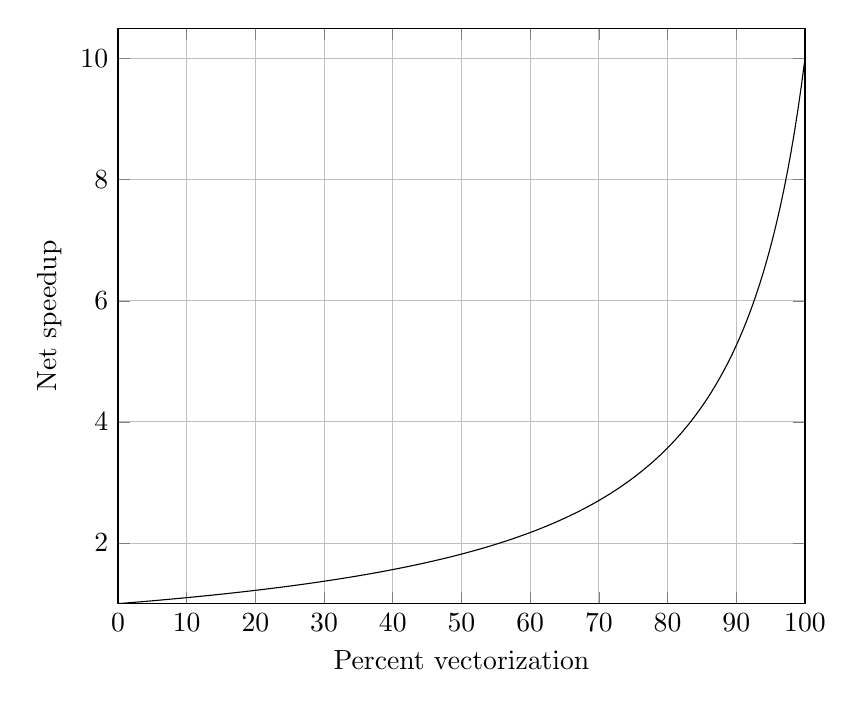
\begin{tikzpicture}
\begin{axis}[
    width=0.85\textwidth,
    xlabel={Percent vectorization},
    ylabel={Net speedup},
    xmin=0, xmax=100,
    ymin=1, ymax=10.5,
    grid=both,
]
\addplot[domain=0:100,samples=200]
{1/( (1 - x/100) + (x/100)/10 )};
\end{axis}
\end{tikzpicture}
\end{center}

\subproblem{b}
Solve $S(p)=2$:
\[
\frac{1}{(1-p)+p/10}=2
\Rightarrow (1-p)+\frac{p}{10}=\frac{1}{2}
\Rightarrow 1-0.9p=\frac{1}{2}
\Rightarrow p=\frac{5}{9}\approx 0.5556.
\]
So \(\boxed{55.56\%}\) vectorization is needed.

\subproblem{c}
If $S=2$ and $p=5/9$, the fraction of \emph{new runtime} spent in vector mode is
\[
\frac{(p/10)}{(1-p)+p/10}
=\frac{p/10}{1/2}
= \frac{p}{5}
=\frac{1}{9}\approx 0.1111.
\]
So \(\boxed{11.11\%}\) of runtime is spent in vector mode after speedup 2 is achieved.

\subproblem{d}
Maximum speedup as $p\to 1$ is $10$. Half of that is $5$.
Solve $S(p)=5$:
\[
\frac{1}{(1-p)+p/10}=5
\Rightarrow (1-p)+p/10=0.2
\Rightarrow 1-0.9p=0.2
\Rightarrow p=\frac{8}{9}\approx 0.8889.
\]
\(\boxed{88.89\%}\) vectorization is needed.

\subproblem{e}
Measured $p=0.70$. If vector hardware improves by an additional $2\times$ beyond $10\times$, then vector speedup becomes $20\times$:
\[
S_{20}=\frac{1}{(1-0.7)+0.7/20}=\frac{1}{0.3+0.035}\approx 2.9851.
\]
Let $p'$ be the vectorization needed to match this speedup with only $10\times$ vector hardware:
\[
\frac{1}{(1-p')+p'/10}=2.9851
\Rightarrow (1-p')+p'/10=\frac{1}{2.9851}\approx 0.335
\Rightarrow 1-0.9p'=0.335
\Rightarrow p'\approx 0.7389.
\]
So the compiler team would need about \(\boxed{73.89\%}\) vectorization (an increase from 70\% to about 73.9\%).

\end{solution}

\problem{6}
\begin{solution}
\subproblem{a}
Instruction count $\text{IC}=150\times 10^6$, frequency $f=2.7$ GHz.
Average CPI:
\[
\text{CPI}=0.5\cdot 3 + 0.3\cdot 4 + 0.2\cdot 5 = 1.5+1.2+1.0=3.7.
\]
Cycles:
\[
\text{Cycles}=150\times 10^6 \cdot 3.7 = 555\times 10^6.
\]
Time:
\[
T=\frac{555\times 10^6}{2.7\times 10^9}\approx 0.2056\ \text{s}.
\]

\subproblem{b}
New design: instructions that were 4 cycles and 5 cycles become 2 cycles; 3-cycle group unchanged.
New CPI:
\[
\text{CPI}'=0.5\cdot 3 + 0.3\cdot 2 + 0.2\cdot 2 = 1.5+0.6+0.4=2.5.
\]
New frequency $f'=2.1$ GHz.
New time:
\[
T'=\frac{150\times 10^6\cdot 2.5}{2.1\times 10^9}
=\frac{375\times 10^6}{2.1\times 10^9}\approx 0.1786\ \text{s}.
\]
Overall percentage improvement:
\[
\frac{T-T'}{T}\times 100\%
=\frac{0.2056-0.1786}{0.2056}\times 100\%
\approx 13.12\%.
\]
So the redesign yields \(\boxed{13.1\%}\) improvement.

\end{solution}

\problem{7}
\begin{solution}
Given CPIs: arithmetic=1, load/store=10, branch=3.
Counts: $N_a=500$M, $N_{ls}=300$M, $N_b=100$M. Total $N=900$M.

Baseline cycles:
\[
C = 500(1)+300(10)+100(3)\ \text{million}
=500+3000+300=3800\ \text{million cycles}.
\]

\subproblem{a}
Reduce arithmetic instruction count by 25\%: $N_a'=0.75\cdot 500=375$M.
New cycles:
\[
C' = 375(1)+300(10)+100(3)=375+3000+300=3675\ \text{million}.
\]
Clock cycle time increases by 10\% (i.e., cycle time $\tau' = 1.1\tau$, or frequency decreases by factor $1/1.1$). Execution time is proportional to cycles $\times$ cycle time:
\[
\frac{T'}{T}=\frac{C'\tau'}{C\tau}=\frac{3675}{3800}\cdot 1.1 \approx 1.063.
\]
So it becomes about \(\boxed{6.3\%}\) slower, hence \textbf{not a good design choice}.

\subproblem{b}
Doubling arithmetic performance: interpret as arithmetic CPI halves from 1 to 0.5.
New cycles:
\[
C_{2\times}=500(0.5)+300(10)+100(3)=250+3000+300=3550\ \text{million}.
\]
Overall speedup:
\[
S_{2\times}=\frac{3800}{3550}\approx 1.070.
\]

If arithmetic is improved by $10\times$: arithmetic CPI becomes $0.1$.
\[
C_{10\times}=500(0.1)+300(10)+100(3)=50+3000+300=3350\ \text{million}.
\]
Speedup:
\[
S_{10\times}=\frac{3800}{3350}\approx 1.134.
\]
So the overall speedups are \(\boxed{1.07\times}\) and \(\boxed{1.13\times}\), respectively.

\end{solution}

\problem{8}
\begin{solution}
Let the unoptimized version have total instruction count $I$ and clock rate $f_u$.
We are told the unoptimized clock rate is 5\% higher than optimized, so
\[
f_u = 1.05 f_o.
\]
In the unoptimized version, 30\% are loads/stores: $0.3I$, and others are $0.7I$.
Optimized executes $2/3$ as many loads/stores, so loads/stores become:
\[
(2/3)\cdot 0.3I = 0.2I,
\]
while other instructions are unchanged ($0.7I$). Thus optimized total instruction count is
\[
I_o = 0.2I+0.7I=0.9I.
\]
All instructions take 1 cycle (CPI=1), so execution times are
\[
T_u = \frac{I}{f_u},\qquad T_o=\frac{0.9I}{f_o}.
\]
Compare:
\[
\frac{T_o}{T_u}=\frac{0.9I/f_o}{I/(1.05f_o)}=0.9\cdot 1.05 = 0.945.
\]
So optimized time is 94.5\% of unoptimized time, i.e.\ \(\boxed{5.5\%}\) faster.
Therefore, \textbf{the optimized version is faster}.

\end{solution}

\problem{9}
\begin{solution}
From the figures, throughput (A,B,C) and power (idle/busy) are:

\begin{itemize}
\item General-purpose (Haswell E5-2699 v3): Throughput A=5482, B=13194, C=12000; Idle=159W, Busy=455W.
\item GPU (NVIDIA K80): Throughput A=13461, B=36465, C=15000; Idle=357W, Busy=991W.
\item TPU: Throughput A=225000, B=280000, C=2000; Idle=290W, Busy=384W.
\end{itemize}

For mixes, treat time as proportional to the sum of weighted reciprocals of throughput:
\[
T \propto \sum_i \frac{w_i}{\text{Throughput}_i},
\]
so speedup of X over Y is \(\frac{T_Y}{T_X}\).

\subproblem{a}
Weights: $w_A=0.7$, $w_B=0.3$ (GPU baseline mix).
\[
T_{\text{GPU}} \propto \frac{0.7}{13461}+\frac{0.3}{36465},\quad
T_{\text{TPU}} \propto \frac{0.7}{225000}+\frac{0.3}{280000}.
\]
Speedup TPU over GPU:
\[
S=\frac{T_{\text{GPU}}}{T_{\text{TPU}}}\approx 14.40.
\]
So \(\boxed{14.4\times}\) speedup.

\subproblem{b}
Using the provided ``\% Max IPS'' per workload, the average achieved percentage is a time-weighted average:
\[
\%\,\text{MaxIPS} = 0.7(\%A)+0.3(\%B).
\]
General-purpose: $0.7(42)+0.3(100)=59.4\%$.

GPU: $0.7(37)+0.3(100)=55.9\%$.

TPU: $0.7(80)+0.3(100)=86.0\%$.

So:
\[
\boxed{\text{Haswell: }59.4\%,\ \text{GPU: }55.9\%,\ \text{TPU: }86.0\%.}
\]

\subproblem{c}
Assume linear power scaling from idle to busy with IPS fraction $\alpha$:
\[
P(\alpha)=P_{\text{idle}}+\alpha(P_{\text{busy}}-P_{\text{idle}}).
\]
Using $\alpha_{\text{GPU}}=0.559$ and $\alpha_{\text{TPU}}=0.86$:
\[
P_{\text{GPU}}\approx 357+0.559(991-357)\approx 711.3\ \text{W},
\]
\[
P_{\text{TPU}}\approx 290+0.86(384-290)\approx 370.8\ \text{W}.
\]
If we take MaxIPS as the max throughput (workload B) for each:
\[
\text{IPS}_{\text{GPU}}\approx 0.559\cdot 36465 \approx 20388,
\quad
\text{IPS}_{\text{TPU}}\approx 0.86\cdot 280000 \approx 240800.
\]
Performance/W:
\[
\frac{\text{IPS}}{W}:\quad
\text{GPU}\approx \frac{20388}{711.3}\approx 28.7,\quad
\text{TPU}\approx \frac{240800}{370.8}\approx 649.4.
\]
Relative performance/W:
\[
\frac{(\text{IPS}/W)_{\text{TPU}}}{(\text{IPS}/W)_{\text{GPU}}}\approx 22.6.
\]
So TPU is about \(\boxed{22.6\times}\) better performance per watt (under these stated assumptions).

\subproblem{d}
Weights: $w_A=0.4$, $w_B=0.1$, $w_C=0.5$.
Compute
\[
T \propto \frac{0.4}{A}+\frac{0.1}{B}+\frac{0.5}{C}.
\]
Speedups relative to general-purpose:
\[
S_{\text{GPU over GP}}\approx 1.86,\qquad
S_{\text{TPU over GP}}\approx 0.485.
\]
Thus the GPU is \(\boxed{1.86\times}\) faster than general-purpose on this mix, while the TPU is \(\boxed{0.485\times}\) due to poor workload C throughput.

\subproblem{e}
A cooling door dissipates 14 kW. Using TDP as the heat to remove:
\[
\#=\left\lfloor \frac{14000}{\text{TDP}}\right\rfloor.
\]
Haswell: $\lfloor 14000/504\rfloor=27$.

NVIDIA K80: $\lfloor 14000/1838\rfloor=7$.

TPU: $\lfloor 14000/861\rfloor=16$.

So \(\boxed{27\ \text{Haswell},\ 7\ \text{K80},\ 16\ \text{TPU}}\).

\subproblem{f}
Power density limit: $200$ W/ft$^2$ and rack area $11$ ft$^2$, so rack budget is
\[
P_{\text{rack,max}}=200\cdot 11 = 2200\ \text{W}.
\]
Servers per rack:
\[
\left\lfloor \frac{2200}{\text{TDP}}\right\rfloor.
\]
Haswell: $\lfloor 2200/504\rfloor=4$.

K80: $\lfloor 2200/1838\rfloor=1$.

TPU: $\lfloor 2200/861\rfloor=2$.

Each rack at this limit dissipates at most 2.2 kW, which is less than a 14 kW cooling door, so \(\boxed{1}\) cooling door is sufficient per such rack.

\end{solution}

\problem{10}
\begin{solution}
\subproblem{a}
Using Moore's Law as doubling every 2 years, from 2015 to 2025 is 10 years, i.e.\ 5 doublings:
\[
2^{10/2}=2^5=32.
\]
So \(\boxed{32\times}\) as many transistors.

\subproblem{b}
Assuming performance continued to improve at a typical 1990s rate of about 52\% per year, from 1978 (VAX-11/780 era) to 2025 is 47 years:
\[
\text{Perf factor} \approx 1.52^{47}\approx 3.5\times 10^8.
\]
So chips would be on the order of \(\boxed{\sim 3\times 10^8}\) times faster than the VAX-11/780 under that formulated continuation.

\subproblem{c}
Clock rate growth has been limited primarily by power/thermal constraints (the power wall), plus diminishing benefits from voltage scaling and increasing wire/interconnect effects.
Architects use the extra transistors to increase performance via parallelism and efficiency: more cores, larger and more sophisticated cache hierarchies, wider SIMD/vector units, specialized accelerators, and microarchitectural techniques that improve IPC rather than raw frequency.

\end{solution}

\end{document}
